\documentclass[a4paper,12pt]{article} 
\usepackage[T2A]{fontenc}			
\usepackage[utf8]{inputenc}			
\usepackage[english,russian]{babel}	
\usepackage{amsmath,amsfonts,amssymb,amsthm,mathtools} 
\usepackage[colorlinks, linkcolor = blue]{hyperref}
\usepackage{upgreek}
\usepackage[left=2cm,right=2cm,top=2cm,bottom=3cm,bindingoffset=0cm]{geometry}
\usepackage{multirow}
\usepackage{graphicx}
\usepackage{xcolor}
\usepackage{multirow}
\usepackage{pgfplots}
\usepackage{pgfplotstable}
\pgfplotsset{compat=1.9}

\pgfplotstableset{ %
        create on use/SquareLight/.style={
                create col/expr={\thisrow{Dark}}}
}

\author{Шелихов Дмитрий\\Группа Б01-305}

\title{\textbf{Работа 3.1.3\\Измерение магнитного поля Земли}} 
\date{\today}

\begin{document} 

\maketitle

\textbf{Цель работы:} исследовать свойства постоянных неодимовых магнитов; измерить с их помощью горизонтальную и вертикальную составляющие индукции магнитного поля Земли и магнитное наклонение.
\par
\textbf{В работе используются:} неодимовые магниты; тонкая нить для изготовления крутильного маятника; медная проволока; электронные весы; секундомер; измеритель магнитной индукции; штангенциркуль; брусок; линейка и штатив из немагнитных материалов; набор гирь и разновесов.\\
\noindent\textbf{Теоретическая справка}

$$ \vec{m} = I\vec{S} \text{ (1) - магнитный момент тонкого витка с током.} $$
$$ \vec {B_{дип}} = \frac {\mu_0}{4\pi}(\frac {3(\vec {m} \cdot \vec{r})\vec{r}}{r^5} - \frac {\vec{m}}{r^3}) \text{ (2) - Магнитное поле точечного диполя.} $$ 
$$ \vec{M} = [\vec{m} \times \vec{B}] \text{ (3) - Механический момент сил, действующий на точечный магнитный диполь $\vec{m}$.} $$
$$ W = -(\vec{m} \cdot \vec{B})  \text{ (4) - Потенциальная энергия, которой обладает диполь с постоянным $\vec{m}$.} $$
$$ \vec{F} = (\vec{m} \cdot \nabla)\vec{B}  \text{ (5) - Сила, действующая на магнитный диполь в неоднородном внешнем поле $\vec{B}$.} $$
$$ F_{12} = -\frac {6m_1m_2}{r^4}  \text{ (6.1) - Сила, взаимодействия двух точечных диполей, \\когда их моменты направлены вдоль соединяющей их прямой.} $$
$$ F_{12} = \frac {3m_1m_2}{r^4}  \text{ (6.2) - Сила, взаимодействия, \\если моменты направлены перпендикулярно соединяющей их прямой.}$$

\noindent\textbf{Экспериментальная установка}

Используем неодимовые шарообразные магниты: \\a) Вещество магнитожёстко\\б) Шары намагничены однородно

$$ \vec {B_0} = \frac {\mu_0 \vec{m}}{2\pi R^3} $$ (7) - магнитное поле внутри шара (однородно).
$$ \vec {m} = \vec{M}V $$ (8), где $\vec{M}$ - намагниченность материала магнита.
$$ \vec {B_r} = 4\pi\vec{M}  $$ (9) - остаточная индукция материала. 
$$ B_p = B_0 = \frac {2}{3}B_r  $$ (10) - индукция на полюсах однородно намагниченного шара. 

\noindent\textbf{Определение магнитного момента магнитных шариков}

\textbf{Метод А.} 

Когда векторы двух магнитных моментов ориентированы вертикально: $$ \vec{m} = \sqrt{\frac{mg{r_{max}^4}}{6}} $$ (11) 

\center{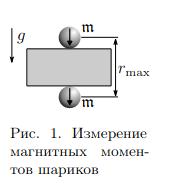
\includegraphics{1.png}}

\textbf{Метод Б.}

Максимальная сила сцепления определется по весу магнитной цепочки, которую способен удержать самый верхний магнитный шарик.

\center{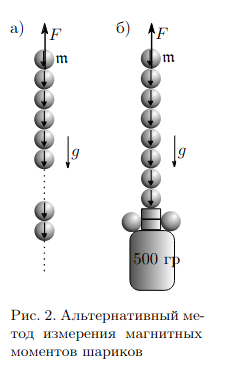
\includegraphics{2.png}}

Сила сцепления двух одинаковых шаров радиусами R с магнитными моментами $\vec{m}$ равна $$ F_0 = \frac{6m^2}{{(2R)}^4} = \frac{3m^2}{8R^4} $$ (12)

Минимальный вес цепочки, при котором она оторвётся от верхнего шарика, равен: $$ F = F_0(1 + \frac{1}{2^4} + \frac{1}{3^4} + \frac{1}{4^4} + ...) \approx 1,08F_0 $$ (13)

\textbf{Измерение горизонтальной составляющей индукции магнитного поля Земли}

Магнитное поле измеряем по периоду крутильных колебаний "магнитной стрелки" вокруг вертикальной оси. Стрелка стремится повернуться по горизонатльной составляющей магнитного поля Земли $\vec{B_{||}}$ в направлении Юг-Север. 

\center{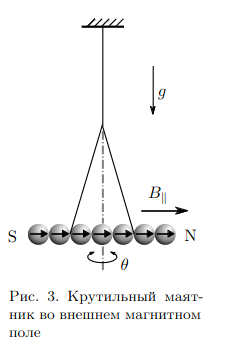
\includegraphics{3.png}}

$$ M = -m_nB_{||}sin\theta $$ (14)  - возвращающий момент сил. 

$$ J_n{\ddot{\theta}} + m_nB_{||}\theta = 0 $$ (15) - уравнение малых колебаний. 

$$ T = 2\pi \sqrt{\frac{J_n}{m_nB_{||}}}  $$ (16) - период малых колебаний. 

$$ J_n \approx \frac{1}{12}m_n{l_n}^2 = \frac{1}{3}n^3mR^2  $$ (17) - момент инерции магнитной стрелки. 

$$ T_n = 2\pi\sqrt{\frac{mR^2}{3mB_{||}}} \cdot n $$ (18) - период колебаний пропорционален числу шаров n, составляющих "стрелку". 

\textbf{Измерение вертикальной составляющей индукции магнитного поля Земли. Магнитное наклонение}

Подвешиваем стрелку в одной точке. $\beta$ - магнитное наклонение

С помощью доп. груза выравниваем стрелку по горизонтали.  

$$ M_n = m_{гр}gr_{гр} = nmB_{\perp}  $$ (19) - момент силы тяжести, уравновешивающего груза. 
Из равенства (19) определяем вертикальную составляющую индукции магнитного поля Земли. 

\center{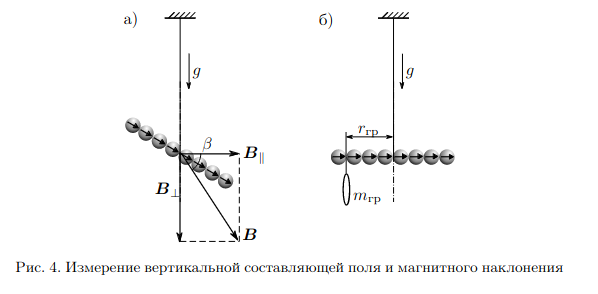
\includegraphics{4.png}}  

\textbf{Ход работы}

I. Определение магнитного момента, намагниченности и остаточной магнитной индукции вещества магнитных шариков. 

1) Измерим диаметр шариков и их массу.

\begin{center}
\begin{tabular}{|c|c|c|}
	\hline
	M, г (76 шаров) & m, г & $\Delta m$, г \\
	\hline
	63,316 & 0,833 & 0,001 \\
	\hline
\end{tabular}
\end{center}
\qquad
\begin{center}
\begin{tabular}{|c|c|}
	\hline
	& d, мм \\
	\hline
	& 5,496 \\
	\hline
	& 5,487 \\
	\hline
	& 5,492 \\
	\hline
	<d>, мм & 5,492 \\
	\hline
	$\Delta$ d, мм & 0,004 \\
	\hline
	d, мм & 5,492 $\pm$ 0,004 \\
	\hline
\end{tabular}
\end{center}

2) С помощью магнитометра измерим индукцию поля $B_p$ на полюсах шарика 

\begin{center}
\begin{tabular}{|c|c|}
	\hline
	N & $B_p$, мТл \\
	\hline
	1 & 357 \\
	\hline
	2 & 319 \\
	\hline
	3 & 275 \\
	\hline
	4 & 305 \\
	\hline
	5 & 346 \\
	\hline
	6 & 265 \\
	\hline
	7 & 368 \\
	\hline
	8 & 367 \\
	\hline
	9 & 357 \\
	\hline
	10 & 354 \\
	\hline
	11 & 400 \\
	\hline
	12 & 393 \\
	\hline
	<$B_p$>, мТл & 342 \\
	\hline
	$\sigma_{B_p}$, мТл & 41 \\
	\hline
	$B_p$, мТл & 342 $\pm$ 41 \\
	\hline
\end{tabular}
\end{center}

3) Определим максимальное расстояние $r_{max}$, на котором шарики удерживают друг друга в поле тяжести Земли.

\begin{center}
\begin{tabular}{|c|c|}
	\hline
	N & $r_{max}$, мм \\
	\hline
	1 & 22,5 \\
	\hline
	2 & 21,0 \\
	\hline
	3 & 22,5 \\
	\hline
	4 & 21,5 \\
	\hline
	5 & 22,5 \\
	\hline
	6 & 21,5 \\
	\hline
	7 & 19,0 \\
	\hline
	8 & 22,0 \\
	\hline
	9 & 21,5 \\
	\hline
	10 & 23,0 \\
	\hline
	<$r_{max}$>, мм & 21,7 \\
	\hline
	$\sigma_{r_{max}}$, мм & 1,1\\
	\hline
	$r_{max}$, мм & 21,7 $\pm$ 1,2 \\
	\hline
\end{tabular}
\end{center}

4) Рассчитаем величину магнитного момента магнитика m по формуле (11). Оценим погрешность 

$$ \varepsilon_m = \frac{1}{2}(\varepsilon_m + 4\varepsilon_{r_{max}})  $$

\begin{center}
\begin{tabular}{|c|c|c|c|c|}
	\hline
	m, г & g, $\frac{см}{с^2}$ & $r_{max}, см$ & m, ед.СГС & $\Delta$m, ед.СГС \\
	\hline
	0,833 & 981,5 & 2,17 & 54,95 & 6,11 \\
	\hline
\end{tabular}
\end{center}

5-6) Используя дополнительные шарики, составим цепочку из 23 шариков и подсоединим цепочку к гире и разновесам так, чтобы общая масса системы составила ~ 500 г. Подберём минимальный вес системы цепочки с гирей, при котором она отрывается от верхнего шарика. Оценить максимальную нагрузку таким методом получилось с точностью до 20 грамм.  

\begin{center}
\begin{tabular}{|c|c|c|c|c|}
	\hline
	$M_{нагр}, г$ &  N, шт & $M_{цеп}, г$ & $M_{общ}, г$ & $\Delta$M \\
	\hline
	539 & 23 & 19,16 & 558 & 20 \\
	\hline
\end{tabular}
\end{center}

7) Рассчитаем силу сцепления двух шаров и по ней определим магнитный момент шарика $\vec{m}$. Оценим погрешность результата по формуле $$ \varepsilon_m = \frac{1}{2} \cdot (\varepsilon_{M_{общ}} + 4 \cdot \varepsilon_d) $$

\begin{center}
\begin{tabular}{|c|c|c|c|c|c|c|}
	\hline
	$M_{общ}, г$ & g, см/$c^2$ & d, см & m, ед.СГС & $\varepsilon_{M_{общ}}$ & $\varepsilon_d$ & $\Delta$m, ед.СГС \\
	\hline
	557,03 & 981,5 & 0,5492 & 87,61 & 0,036 & 7,3 $\cdot 10^{-4}$ & 3,13 \\
	\hline
\end{tabular}
\end{center}

8) Итого, мы получили два различных значения магнитных моментов: 
\begin{center}
\begin{tabular}{|c|c|}
	\hline
	Способ А & Способ Б \\
	\hline
	m = (54,95 $\pm$ 6,11) ед.СГС & m = (87,61 $\pm$ 3,13) ед.СГС \\
	\hline
\end{tabular}
\end{center}

Исходя из полученных данных второй метод обладает меньшей погрешностью. 
По табличным данным для данного материала остаточная индукция $B_r$ = 12200 Гаусс, что соответствует m = 85 ед.СГСЭ для шариков диаметром d = 5,5 мм. 
Исходя из этого, далее будем считать правильными данные, полученные в методе Б.

9) Рассчитаем величину намагниченности материала шариков M и остаточную индукцию магнитного поля $B_r$. Проведем сравнение с табличными значеними. 

\begin{center}
\begin{tabular}{|c|c|c|c|c|c|}
	\hline
	d, мм & V, мм3 & m, ед.СГС & M, ед.СГС & $B_r$, кГс & $B_{r_{табл}}$, кГс \\
	\hline
	5,492 $\pm$ 0,004 & 86,734 $\pm$ 0,190 & 87,61 $\pm$ 3,13 & 1010 $\pm$ 10 & 12,7 $\pm$ 0,1 & 12,2-12,5\\
	\hline
\end{tabular}
\end{center}

Видим, что полученные данные отличаются от табличных всего на 0.8 - 5\%. Это подтверждает, что метод Б более точный, чем метод А. Незначительное расхождение с табличным значением может быть вызвано отличием магнитного момента $\vec{m}$ самого верхнего шарика цепочки от среднего значения. Это различие может достигать 12\%! Опыт следовало проводить меняя верхний шарик местами с другими шариками цепи, усредняя магнитный момент шарика сверху.

10) Рассчитаем индукцию $B_p$ у полюсов шарика. Сравним рассчётное значение $B_p$ с измеренным.

\begin{center}
\begin{tabular}{|c|c|}
	\hline
	$B_{p_{измеренное}}$, мТл & $B_{p_{рассчётное}}$, мТл \\
	\hline
	342 $\pm$ 41 & 84,7 $\pm$ 0,7 \\ 
	\hline
\end{tabular}
\end{center}

II. Определение горизонтальной составляющей магнитного поля Земли

11) Соберём крутильный маятник из 12 магнитных шариков и подвесим его на немагнитном штативе. Используя $\Lambda$-образный подвес, установим "магнитную стрелку " в горизонтальное положение.

\center{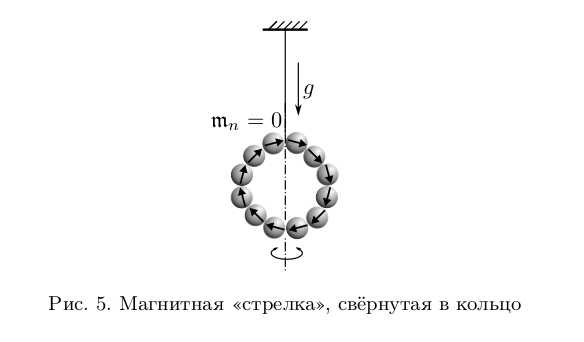
\includegraphics{5.png}}

12-13) Возбудим крутильные колебания маятника вокруг вертикальной оси и определим их период. Оценим влияние упругости (модуля кручения) нити на период колебаний, возбудив крутильные колебания "стрелки", свёрнутой в кольцо (магнитный момент такого кольцеобразного маятника равен 0). Исследуем зависимость периода T крутильных колебаний "стрелки" от количества магнитных шариков n, составляющих "стрелку". Измерения проведем для значений n = 3, 4, 5 ..., 12. Причем каждый раз перед измерением будем выставлять стрелку горизонтально. 

\begin{center}
\begin{tabular}{|c|c|c|c|}
	\hline
	n, шт & t, c & $n_{колеб}$, шт & T, c \\
	\hline
	\multirow{5}{*}{12} & 18,47 & 5 & 3,69 \\
	\cline{2-4} & 18,31 & 5 & 3,66 \\
	\cline{2-4} & 17,94 & 5 & 3,59 \\
	\cline{2-4} & 18,12 & 5 & 3,62 \\
	\cline{2-4} & 18,28 & 5 & 3,66 \\
	\hline
	\multicolumn{4}{|c|}{T = (3,64 $\pm$ 0,04) c} \\
	\hline
	\multirow{6}{*}{11} & 17,31 & 5 & 3,46 \\
	\cline{2-4} & 17,06 & 5 & 3,41 \\
	\cline{2-4} & 17,13 & 5 & 3,43 \\
	\cline{2-4} & 17,09 & 5 & 3,42 \\
	\cline{2-4} & 17,28 & 5 & 3,46 \\
	\cline{2-4} & 16,87 & 5 & 3,37 \\
	\hline
	\multicolumn{4}{|c|}{T = (3,42 $\pm$ 0,03) c} \\
	\hline
	\multirow{7}{*}{10} & 15,35 & 5 & 3,07 \\
	\cline{2-4} & 15,31 & 5 & 3,06 \\
	\cline{2-4} & 15,31 & 5 & 3,06 \\
	\cline{2-4} & 15,29 & 5 & 3,05 \\
	\cline{2-4} & 15,25 & 5 & 3,05 \\
	\cline{2-4} & 15,59 & 5 & 3,12 \\
	\cline{2-4} & 15,56 & 5 & 3,11 \\	
	\hline
	\multicolumn{4}{|c|}{T = (3,08 $\pm$ 0,03) c} \\
	\hline
	\multirow{6}{*}{9} & 14,03 & 5 & 2,81 \\
	\cline{2-4} & 14,28 & 5 & 2,86 \\
	\cline{2-4} & 13,97 & 5 & 2,79 \\
	\cline{2-4} & 14,28 & 5 & 2,86 \\
	\cline{2-4} & 14,38 & 5 & 2,88 \\
	\cline{2-4} & 14,16 & 5 & 2,83 \\
	\hline
	\multicolumn{4}{|c|}{T = (2,84 $\pm$ 0,03) c} \\
	\hline
	\multirow{6}{*}{8} & 12,81 & 5 & 2,56 \\
	\cline{2-4} & 12,54 & 5 & 2,51 \\
	\cline{2-4} & 12,62 & 5 & 2,52 \\
	\cline{2-4} & 12,59 & 5 & 2,52 \\
	\cline{2-4} & 12,87 & 5 & 2,57 \\
	\cline{2-4} & 12,78 & 5 & 2,56 \\
	\hline
	\multicolumn{4}{|c|}{T = (2,54 $\pm$ 0,02) c} \\
	\hline
\end{tabular}
\end{center}

\qquad

\begin{center}
 \begin{tabular}{|c|c|c|c|}
     \hline
     n, шт & t, c & $n_{колеб}$, шт & T, c \\
     \hline
     \multirow{6}{*}{7} & 11,62 & 5 & 2,32 \\
     \cline{2-4} & 11,81 & 5 & 2,36 \\
     \cline{2-4} & 11,66 & 5 & 2,33 \\
     \cline{2-4} & 11,90 & 5 & 2,38 \\
     \cline{2-4} & 11,84 & 5 & 2,37 \\
     \cline{2-4} & 11,87 & 5 & 2,37 \\
     \hline
     \multicolumn{4}{|c|}{T = (2,36 $\pm$ 0,02) c} \\
     \hline
     \multirow{8}{*}{6} & 10,84 & 5 & 2,17 \\
     \cline{2-4} & 10,94 & 5 & 2,19 \\
     \cline{2-4} & 10,69 & 5 & 2,14 \\
     \cline{2-4} & 10,84 & 5 & 2,17 \\
     \cline{2-4} & 10,63 & 5 & 2,13 \\
     \cline{2-4} & 10,75 & 5 & 2,15 \\
     \cline{2-4} & 10,94 & 5 & 2,19 \\
     \hline
     \multicolumn{4}{|c|}{T = (2,16 $\pm$ 0,02) c} \\
     \hline
     \multirow{6}{*}{5} & 9,50 & 5 & 1,90 \\
     \cline{2-4} & 9,40 & 5 & 1,88 \\
     \cline{2-4} & 9,47 & 5 & 1,89 \\
     \cline{2-4} & 9,66 & 5 & 1,93 \\
     \cline{2-4} & 9,47 & 5 & 1,89 \\
     \cline{2-4} & 9,57 & 5 & 1,91 \\
     \hline
     \multicolumn{4}{|c|}{T = (1,90 $\pm$ 0,02) c} \\
     \hline
     \multirow{6}{*}{4} & 7,69 & 5 & 1,54 \\
     \cline{2-4} & 7,93 & 5 & 1,59 \\
     \cline{2-4} & 7,78 & 5 & 1,56 \\
     \cline{2-4} & 7,88 & 5 & 1,58 \\
     \cline{2-4} & 7,69 & 5 & 1,54 \\
     \cline{2-4} & 7,75 & 5 & 1,55 \\
     \hline
     \multicolumn{4}{|c|}{T = (1,56 $\pm$ 0,02) c} \\
     \hline
     \multirow{6}{*}{3} & 6,13 & 5 & 1,23 \\
     \cline{2-4} & 6,13 & 5 & 1,23 \\
     \cline{2-4} & 6,07 & 5 & 1,21 \\
     \cline{2-4} & 6,07 & 5 & 1,21 \\
     \cline{2-4} & 6,31 & 5 & 1,26 \\
     \cline{2-4} & 6,18 & 5 & 1,24 \\
     \hline
     \multicolumn{4}{|c|}{T = (1,23 $\pm$ 0,02) c} \\
     \hline
\end{tabular}
\end{center}

\begin{center}
\begin{tabular}{|c|c|c|c|}
	\hline
	& t, c & $N_{колеб}$, шт & T, c \\
	\hline
	Кольцо из n = 12 шариков & 61 & 5 & 12,02 \\
	\hline
\end{tabular}
\end{center}

Таким образом период колебаний, вызванных наличием упругости нити, не менее чем в 3 раза больше периода колебаний магнитной стрелки. Поэтому в дальнейших расчётах колебаний пренебрежем упругостью нити.
 
14) Построим график экспериментальной зависимости T(n).

\pgfplotstableread{
x	y 		y-max 	y-min
3	1.23	0.02	0.02
4	1.56	0.02	0.02
5	1.90	0.02	0.02
6	2.16	0.02	0.02
7	2.36	0.02	0.02
8	2.54	0.02	0.02
9	2.84	0.03	0.03
10	3.08	0.03	0.03
11	3.42	0.03	0.03
12	3.64	0.04	0.04
}{\mytable}

\begin{tikzpicture}
\begin{axis} [
	title = T(n),
	xlabel = {$n$, шт},
	ylabel = {$T$, с},
	minor tick num = 2
]

\addplot +[mark options = {scale = 0.1,}]
	plot [error bars/.cd, y dir=both, y explicit]
	table [y error plus=y-max, y error minus=y-min] {\mytable};

\addplot +[mark options = {scale = 0,}]
	table[row sep=\\,				%аппроксимация
    y={create col/linear regression={y=Y}}]
    {
    	X Y\\
		3   1.23\\   
		4   1.56\\    
		5   1.90\\   
		6   2.16\\   
		7   2.36\\  
		8   2.54\\    
		9   2.84\\   
		10  3.08\\   
		11  3.42\\    
		12  3.64\\  
    };
	\addlegendentry{
        k$\approx \pgfmathprintnumber{\pgfplotstableregressiona}$} 
\end{axis}
\end{tikzpicture}

Видим, что зависимость линейна. По значению углового коэффициента рассчитаем величину горизонтальной составляющей магнитного поля Земли.

$$ k = 2\pi\sqrt{\frac{mR^2}{3|\vec{m}|B_{||}}} $$

\begin{center}
\begin{tabular}{|c|c|c|c|c|}
	\hline
	m, г & R, см & |$\vec{m}$|, ед.СГС & k, c & $B_{||}$, Гс \\
	\hline
	0,833 $\pm$ 0,001 & 0,2746 $\pm$ 0,0002 & 87,61 $\pm$ 3,13 & 0,26 & 0,140 $\pm$ 0,005\\
	\hline
\end{tabular}
\end{center}

III. Определение вертикальной составлящей магнитного поля Земли.

15) Изготовим магнитную "стрелку" из n = 10 шариков и подвесим её за середину с помощью нити на штативе.

16) Определим механический момент сил, действующий со стороны магнитного поля Земли на горизонтально расположенную магнитную "стрелку". Для этого, с помощью одного или нескольких кусочков проволоки, уравновесим "стрелку" в горизонтальном положении. 

17-18) С помощью весов определим массу уравновешивающего груза $m_{гр}$. Из условия равновесия рассчитаем механический момент сил M, действующих на горизонтальную стрелку со стороны поля Земли. Измерение момента сил проведем для четных значений n = 4,6,8,10,12.

$$ M_n = m_{гр}gr_{гр}  $$	

\begin{center}
\begin{tabular}{|c|c|c|c|c|c|}
	\hline
	n, шт & $r_{гр}$, см & $m_{гр}$, г & g, $\frac{cm}{c^2}$ & ${M_n}^i$, дин$\cdot$см & $M_n$, дин$\cdot$см\\
	\hline
	\multirow{4}{*}{12} & 2,746 & 0,194 & \multirow{13}{*}{981,5} & 522,87 & \multirow{4}{*}{515,73 $\pm$ 10,08}\\
	\cline{2-3}\cline{5-5} 		& 2,197 & 0,240 &  & 517,48 & \\
	\cline{2-3}\cline{5-5} 		& 1,648 & 0,311 &  & 502,92 & \\
	\cline{2-3}\cline{5-5} 		& 1,098 & 0,482 &  & 519,63 & \\
	\cline{1-3}\cline{5-6}
	\multirow{3}{*}{10} & 1,648 & 0,257 &  & 415,60 & \multirow{3}{*}{428,54 $\pm$ 11,68}\\
	\cline{2-3}\cline{5-5}      & 1,098 & 0,407 &  & 438,78 & \\
    \cline{2-3}\cline{5-5}      & 0,549 & 0,800 &  & 431,23 & \\
    \cline{1-3}\cline{5-6}
    \multirow{3}{*}{8} & 1,648 & 0,190 &  & 307,25 & \multirow{3}{*}{325,94 $\pm$ 14,75}\\
    \cline{2-3}\cline{5-5}      & 1,098 & 0,311 &  & 335,28 & \\
    \cline{2-3}\cline{5-5}      & 0,549 & 0,622 &  & 335,28 & \\
   	\cline{1-3}\cline{5-6}
   	\multirow{2}{*}{6} & 1,098 & 0,284 &  & 306,17 & \multirow{2}{*}{313,72 $\pm$ 9,03}\\
    \cline{2-3}\cline{5-5}      & 0,549 & 0,596 &  & 321,27 & \\
	\cline{1-3}\cline{5-6}
	4 & 0,549 & 0,286 & & 154,11 & 154,11 $\pm$ 3,78 \\
	\hline
\end{tabular}
\end{center}

19) Построим график экспериментальной зависимости M(n).

\pgfplotstableread{
x	y 		y-max 	y-min
12	515.73	10.08	10.08
10	428.54	11.68	11.68
8	325.94	14.75	14.75
6	313.72	9.03	9.03
4	154.11	4.51	4.51
}{\mytable}

\begin{tikzpicture}
\begin{axis} [
	title = M(n),
	xlabel = {$n$, шт},
	ylabel = {$M$, дин$\cdot$см},
	minor tick num = 2
]

\addplot +[mark options = {scale = 0.1,}]
	plot [error bars/.cd, y dir=both, y explicit]
	table [y error plus=y-max, y error minus=y-min] {\mytable};

\addplot +[mark options = {scale = 0,}]
	table[row sep=\\,				%аппроксимация
    y={create col/linear regression={y=Y}}]
    {
    	X Y\\
		12   515.73\\   
    	10   428.54\\
		8    325.94\\
		6    313.72\\
		4    154.11\\
    };
	\addlegendentry{
        k$\approx \pgfmathprintnumber{\pgfplotstableregressiona}$} 
\end{axis}
\end{tikzpicture}

Исходя из линейной аппроксимации k$\approx$41,9 дин$\cdot$см. По значению углового коэффициента k рассчитаем величину вертикальной составляющей $B_{\perp}$ магнитного поля Земли. Оценим погрешность результата.

\begin{center}
\begin{tabular}{|c|c|c|}
	\hline
	k, дин$\cdot$см & m, ед.СГС & $B_{perp}$, Гс \\
	\hline
	41,9 $\pm$ 0,8 & 87,61 $\pm$ 3,13 & 0,48 $\pm$ 0,03 \\
	\hline
\end{tabular}
\end{center}

20) Используя результаты измерения $B_{||}$ и $B_{\perp}$, определим магнитное наклонение $\beta$ и полную величину индукции магнитного поля Земли на широте Долгопрудного.

$$ B_{полн} = \sqrt{{B_{||}}^2+{B_{\perp}}^2} $$
$$ \beta = arctg\frac{B_{\perp}}{B_{||}}$$

\begin{center}
\begin{tabular}{|c|c|c|c|}
	\hline
	$B_{||}$, Гс & $B_{\perp}$, Гс & $B_{полн}$, Гс & $\beta$ \\
	\hline
	0,140 $\pm$ 0,005 & 0,48 $\pm$ 0,03 & 0,50 $\pm$ 0,03 & 74 $\pm$ 4\\
	\hline
\end{tabular}
\end{center}

21) 

\end{document}

